\subsection{Problema a resolver}

El siguiente ejercicio se da en el contexto de un museo donde se requiere, por cuestiones de seguridad, colocar sensores de forma tal que todo el piso esté cubierto por los lásers que estos emiten. Existen dos tipos de sensores: los bidireccionales (que emiten señales horizontales o verticales) y los cuatridireccionales (que emiten señales verticales y horizontales). Los precios de éstos son \$4000 y \$6000 respectivamente. Se pide, también, que un sensor no apunte hacia otro dado que esto podría dejarlos sin funcionar. Además, se pide que ciertos lugares, definidos como \textit{importantes}, sean atravesados por dos lásers simultáneamente. El objetivo del algoritmo a realizar consiste en encontrar una forma de colocar los sensores de manera que el suelo quede completamente cubierto y que los lugares \textit{importantes} estén atravesados por un láser horizontal y otro vertical utilizando el mínimo costo posible. Por otra parte, debe ser tenido en cuenta que el museo cuenta con paredes que pueden interferir los lásers de los sensores.\newline

\newline
\textbf {Formatos de entrada y salida:}\newline
\newline
La entrada del algoritmo contiene una instancia del problema. La primera línea indica las dimensiones $n$ y $m$ de la grilla. A esta línea le siguen $n$ líneas, cada una con $m$ valores separados por espacios, indicando el contenido de cada una de las $n$ x $m$ casillas de la grilla, donde un 0 representa una pared, un 1 representa un casillero libre común y un 2 representa un casillero libre importante.\newline

En el caso en el que el problema no tenga solución, la salida deberá contener únicamente una línea con el valor -1. Caso contrario, la salida debe comenzar con dos números enteros: 
$$S\ C$$ 
donde $S$ es la cantidad de sensores utilizados y $C$ es el costo total de la solución. Luego, para cada sensor utilizado, debe haber una línea con el siguiente formato: 
$$t\ f\ c$$ 
donde $t$ es el tipo de sensor y $(f,c)$ son la fila y columna en donde éste se ubica (la esquina superior izquierda de la grilla es la posición (1,1) y la inferior derecha es la $(n,m)$). Para los sensores cuatridireccionales, $t$ debe valer 1, para los bidireccionales en forma horizontal $t$ debe valer 2 y en forma vertical 3.\newline
\newline
Dos ejemplos de este problema son los siguientes:

\begin{itemize}
\item {\large{\textbf{Ejemplo 1:}}}

\begin{figure}[H] % indico que voy a poner una figura y [h] indica que la posición relativa, tambien puedo usar t = top entre otros.
\hfill
\begin{minipage}[t]{.45\textwidth}
\begin{center}
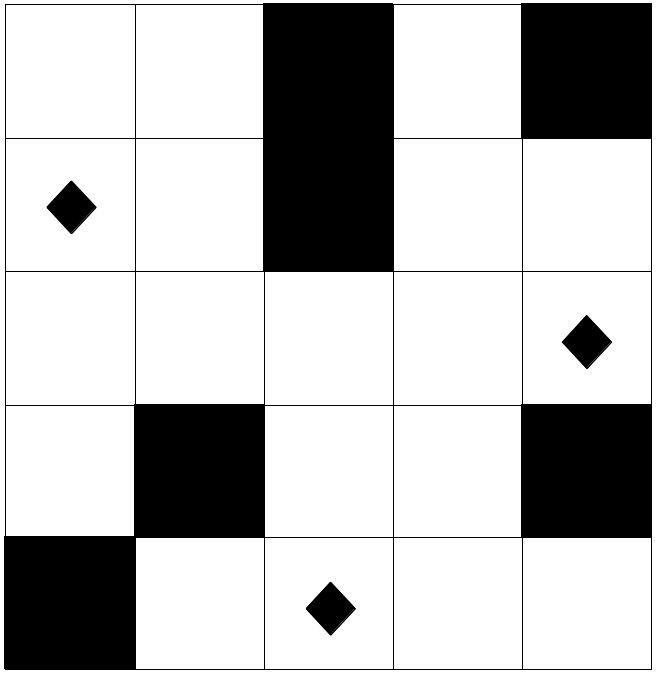
\epsfig{file=ejemplo1_ej3.jpg, scale=0.15} % primera imagen colocada a la izquierda
\caption{Ejemplo de la entrada de un caso con solución.}
\label{fig-tc1}
\end{center}
\end{minipage}
\hfill
\begin{minipage}[t]{.45\textwidth}
\begin{center}
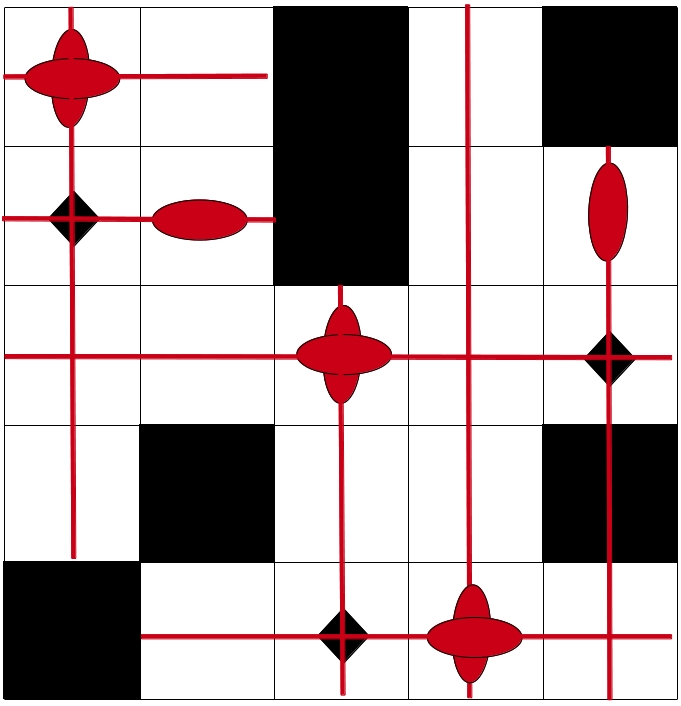
\epsfig{file=solucion_ejemplo1_ej3.jpg, scale=0.15} % segunda imagen colocada a la derecha
\caption{Ejemplo de la salida de un caso con solución.}
\label{fig-tc2}
\end{center}
\end{minipage}
\hfill
\end{figure}

En la Figura 12, puede observarse un ejemplo en el que el suelo del museo se encuentra representado por una cuadrícula. Los cuadros blancos consisten en casillas vacías, los negros representan las paredes y los que tienen un rombo en su interior los lugares importantes. La Figura 13 muestra una posible solución al problema. Las cruces rojas representan los sensores cuatridireccionales y los elipsoides los sensores horizontales y verticales. Los sensores emiten señales láser simbolizadas por líneas rojas.\newline

En este ejemplo, el costo total utilizado es de \$26000.

\textbf{Formato de entrada:} 
$$5\ \ 5$$
$$1\ \ 1\ \ 0\ \ 1\ \ 0$$
$$2\ \ 1\ \ 0\ \ 1\ \ 1$$
$$1\ \ 1\ \ 1\ \ 1\ \ 2$$
$$1\ \ 0\ \ 1\ \ 1\ \ 0$$
$$0\ \ 1\ \ 2\ \ 1\ \ 1$$
\textbf{Formato de salida:} 
$$5\ \ 26000$$
$$1\ \ 0\ \ 0$$
$$2\ \ 1\ \ 1$$
$$3\ \ 1\ \ 4$$
$$1\ \ 2\ \ 2$$
$$1\ \ 4\ \ 3$$

\newline

\item {\large{\textbf{Ejemplo 2:}}}

\begin{center}
\begin{figure}[H] % indico que voy a poner una figura y [h] indica que la posición relativa, tambien puedo usar t = top entre otros.
\begin{minipage}[t]{.45\textwidth}
\begin{center}
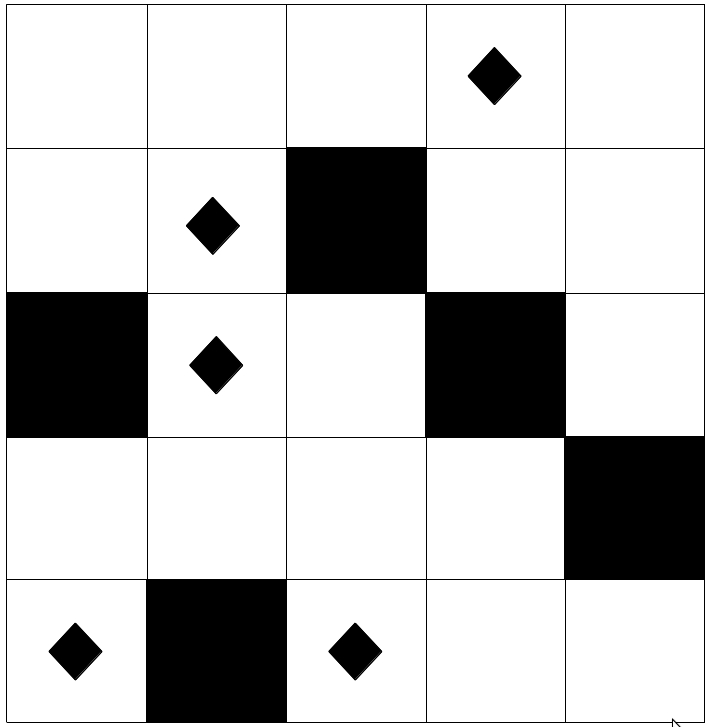
\epsfig{file=ejemplo2_ej3.jpg, scale=0.13} % primera imagen colocada a la izquierda
\caption{Ejemplo de la entrada de un caso sin solución.}
\end{center}
\label{fig-tc1}
\end{minipage}
\end{figure}
\end{center}

En el ejemplo de la Figura 14, se puede observar un caso que no tiene solución. Esto se debe a que la celda (5,1) contiene un casillero importante que debe ser atravesado por dos lásers simultáneamente. Dado que éste se encuentra en una esquina del tablero y posee una pared a su lado, no puede ser atravesado por un láser horizontal.

\textbf{Formato de entrada:} 
$$5\ \ 5$$
$$1\ \ 1\ \ 1\ \ 2\ \ 1$$
$$1\ \ 2\ \ 0\ \ 1\ \ 1$$
$$0\ \ 2\ \ 1\ \ 0\ \ 1$$
$$1\ \ 1\ \ 1\ \ 1\ \ 0$$
$$2\ \ 0\ \ 2\ \ 1\ \ 1$$
\textbf{Formato de salida:} $$-1$$\newline
\end{itemize}

\subsection{Resolución coloquial}

Para resolver el problema presentado decidimos utilizar la técnica de $backtracking$. Ésta consiste en evaluar las posibles combinaciones de soluciones del problema hasta llegar a la deseada. Para ello, definimos criterios de parada que nos permitieran decidir si las soluciones parcialmente obtenidas eran candidatas a soluciones válidas.\newline
\newline
Para lograr una correcta visualización del problema, representamos el piso entero del museo con una matriz, respetando las paredes y las casillas importantes. Luego, cada elemento de la matriz representa a una baldosa/casillero del piso y almacena el estado de la misma. Esto significa que de acuerdo a si contiene un 0, un 1 o un 2, podemos saber si hay algún sensor en ella o si le pasa algún láser por encima.\newline
\newline
Nuestro algoritmo, en primera instancia, genera un árbol de decisiones sobre todas las combinaciones posibles de cada casillero. Para lograrlo, recorre paulatinamente la matriz mencionada y, en cada paso, toma una decisión sobre el casillero actual para avanzar, luego, al siguiente. Las posibles decisiones son colocar o no algún sensor, empezando por intentar con el sensor cuatridireccional, para proseguir con el horizontal, luego el vertical y por último sin ningún sensor. Con el fin de acotar el tiempo de ejecución del algoritmo, se idearon ciertas cotas que frenan la ramificación del nodo que llega a algún caso que no tiene solución. Las cotas implementadas fueron las siguientes:
\begin{enumerate}
\item Una vez que se encuentra una solución, se almacena su costo y cualquier rama cuyo costo actual sea mayor al $almacenado-2000$ (siendo 2000 = diferencia entre un sensor cuatridireccional y uno bidireccional) es descartado.
\item Sobre las casillas importantes no puede haber ningún sensor cuatridireccional ni bidireccional. Esto se debe a que en dicho caso, no existiría la posibilidad de atravesarlo por dos lásers sin que se rompan.
\item No puede haber ningún sensor vertical en las filas que tengan algún casillero importante, lo mismo para sensores horizontales en la columna. Esto se debe al mismo motivo mencionado en el ítem anterior.
\item Cualquier fila conteniendo algún sensor vertical no puede tener ninguno horizontal pues provocará un choque entre ellos. Análogamente de para una columna conteniendo un sensor horizontal a la que se le quiera agregar uno vertical.
\end{enumerate}
De este modo, el árbol realizado contiene en cada nodo una posibilidad de casillero y, como máximo, tres hermanos con las otras posibilidades. Luego, el árbol es recorrido y se comparan los precios de cada solución válida hasta llegar a una mínima.\newline
\newline

El pseudocódigo que describe la solución a nuestro problema es el siguiente:

\begin{algorithm}[H]
	\SetAlgoLined
	\caption{Algoritmo de Backtracking}
	\KwIn{Matriz $grilla$}
	\KwOut{Lista sensores}
	
	Matriz $mejorGrilla$
	Lista $casillasLibres$\\

	\For{Posicion $p \in grilla$}{
		\If{p esta libre}{
			$casillasLibres \leftarrow p$\\
		}
		\If{$p$ es importante}{
			\textbf{RestringirPorImportantes}(p)\\
		}
	}

	sensores := backtrack($grilla$, $casillasLibres$, $mejorGrilla$)\\

	\textbf{devolver} sensores
\end{algorithm}

\begin{algorithm}[H]
	\SetAlgoLined
	\caption{backtrack}
	\KwIn{Matriz $grilla$, Lista $casillasLibres$, Matriz $mejorGrilla$, Entero $mejorCostoObtenido$}
	\KwOut{}

    \If{$costoActual$ > $(mejorCostoObtenido - 2000)$}{
        backtrack($grilla$, $casillasLibres$)\\
	}
	
	\If{$casillasLibres$ esta vacio}{
		\If{chequearSolucion($grilla$) \land $ (costoActual $ < $ mejorCostoObtenido)$}{
			$mejorCostoObtenido$ := $costoActual$\\
			$mejorGrilla$ := $grilla$
		}
    }

	Casilla $casillaActual$ := Proxima casilla \in casillasLibres\\

	\If{$casillaActual$ tiene un laser pasando por ella}{
		backtrack($grilla$,$casillasLibres$,$mejorGrilla$,$mejorCostoObtenido$);
	}
	
	\If{Puedo poner un sensor bidireccional en $casillaActual$}{
		Restringir por láser bidireccional\\
		Saco casillaActual de casillasLibres\\
		backtrack($grilla$, $casillasLibres$)\\
	}
	\If{Puedo poner un sensor vertical en $casillaActual$}{
		restringirPorLaser($casillaActual$,$grilla$)\\
		restringirPorSensor($casillaActual$,$grilla$)\\
		Saco casillaActual de casillasLibres\\
		backtrack($grilla$, $casillasLibres$)\\
	}
	\If{Puedo poner un sensor horizontal en $casillaActual$}{
		restringirPorLaser($casillaActual$,$grilla$)\\
		restringirPorSensor($casillaActual$,$grilla$)\\
		Saco casillaActual de casillasLibres\\
		backtrack($grilla$, $casillasLibres$)\\
	}

	backtrack($grilla$, $casillasLibres$)\\
	$casillasLibres \leftarrow casillaActual$

	\textbf{devolver}
\end{algorithm}

\subsection{Demostración de correctitud}

Para demostrar la correctitud de nuestro algoritmo, debemos probar que se cumplen las siguientes propiedades:
\begin{itemize}
\item Nuestro algoritmo genera todas las combinaciones posibles para cada casillero.
\item Las podas utilizadas no alteran la solución final.
\item La solución es óptima, es decir, no existe otra cuyo costo sea menor.
\end{itemize}

\newline

\textbf{Nuestro algoritmo genera todas las combinaciones posibles para cada casillero.} \newline

Esto ocurre pues, para cada elemento de la matriz mencionada, se evalúan las cuatro posibilidades (sensor horizontal, sensor vertical, sensor cuatridimensional y sin sensor) sin tener en cuenta la decisión de la casilla anterior siempre y cuando el caso no esté contemplado en alguna poda o que no rompa los casos especificados en el enunciado. Luego, todas las combinaciones posibles de casos son generadas.\newline
\newline 

\textbf{Las podas utilizadas no alteran la solución final} \newline

Las podas utilizadas son:
\begin{itemize}
\item Poda sobre el costo : Sea T el costo de la mejor solucion generada por el algoritmo en determinado momento. Si cualquier otra solucion parcial ya alcanza el costo T-2000 pueden pasar dos cosas, o que el costo final sea T-2000 
o que el costo final sea mayor a T $($ya que menos es imposible dado que la diferencia que existe entre los sensores de de 2000 $)$. Luego nuestro algoritmo descarta aquellas soluciones parciales cuyos costos superen los T-2000
asegurando no eliminar soluciones factibles.  
\item Poda sobre casilleros importantes: Esta es trivial, ya que cualquier solucion que un casillero importante contenga un sensor cuatridimencional no va a permitir que ningun otro laser impacte sobre ese casillero.
\item Poda sobre mismas lineas: Esta tambien es trivial, ya que en la misma linea donde tengo un sensor bidireccional vertical no puedo poner una vertical, lo mismo para el sensor bidireccional horizontal. Y donde 
tengo un sensor cuatridimencional, no puedo poner ningun otro sensor en la misma linea.
\item Poda sobre lineas de casilleros importantes: Dado un casillero importante hay que asegurarse que dos lineas atraviesen al mismo, y como solo hay lineas horizontales y verticales, no puede haber soluciones
ddonde haya sensores bidireccionales verticales en los costados (misma linea horizontal) de un casillero importante; y no puede haber sensores verticales arriba o abajo (misma linea vertical) del casillero importante.
 Por lo tanto, esto no solo es una poda, sino una condicion necesaria de la solucion.
\end{itemize}

\textbf{La solución es óptima, es decir, no existe otra cuyo costo sea menor.} \newline

Dado que nuestro algoritmo compara el valor de la solución creada con la más óptima almacenada y, en caso de que el costo de ésta última sea menor reemplaza la más óptima por ésta, el resultado final es la solución con menor costo de entre todas las posibles.


\subsection{Complejidad del algoritmo}

Dado que tenemos $n$x$m$ baldosas de las cuales nuestro algoritmo genera 4 casos distintos para cada una de estas, obtenemos 4$^{nxm}$ combinaciones posibles. A su vez, por cada uno de estos casos se realizan una serie de operaciones, entre las cuales se encuentran:
\begin{itemize}
\item $Colocar\ sensores\ verticales$ y $Restringir\ celdas\ verticales$: Estas funciones en el peor de los casos recorren toda una columna de la matriz por lo cual tienen complejidad $\mathcal{O}(n)$
\item $Colocar\ sensores\ horizontales$ y $Restringir\ celdas\ horizontales$: Estas funciones en el peor de los casos recorren toda una fila de la matriz por lo cual tienen complejidad $\mathcal{O}(m)$
\item $Chequear\ solución$: Esta función recorre toda la matriz para corroborar si esta contiene una solución valida o no por lo que su complejidad es de $\mathcal{O}(nxm)$
\end{itemize}

En los casos en los que se coloca un sensor, o bien se usan las funciones $Colocar\ sensores\ verticales/horizontales$ y $Restringir\ celdas\ horizontales/verticales$ o bien las funciones $Colocar\ sensores\ verticales$ y $Colocar\ sensores\ horizontales$. En ambos casos, estas tienen complejidad $\mathcal{O}(n+m)$ ya que es la suma de las dos complejidades. Por otro lado, en muchos nodos se chequea si la solución a la cual se llego resuelve o no el problema, con lo cual se podría acotar el costo de cada nodo con la complejidad de $chequear\ solución$.

Dicho lo anterior, ya que tenemos 4$^{nxm}$ combinaciones posibles y cada una de estas en el peor de los casos requieren de una complejidad de $\mathcal{O}(nxm)$, nuestro algoritmo tiene un costo de $\mathcal{O}(nxm)$x4$^{nxm}$. Hay que tener en cuenta que a pesar de que la complejidad no lo refleje, las podas cumplen un trabajo fundamental en cuestiones temporales ya que evitan que se generen todos los casos y esto reduce mucho el tiempo de ejecución. Estas podas no impactan de forma positiva en la complejidad del algoritmo ya que si asi lo hicieran dejarían de ser podas y pasarían a constituir un mejor algoritmo.
\subsection{Código fuente}

\begin{figure}[H]
\begin{center}
\begin{verbatim}
for (int i = 0; i < g.size(); ++i) {
   for (int j = 0; j < g[i].size(); ++j) {
      if (g[i][j].tipo == 2)
         restringirCasillasPorImportante(i, j); 
         if (g[i][j].tipo == 1) 
            casillasLibres.push(&(g[i][j]));
         }
      }
\end{verbatim}
\caption{Restringe las casillas segun corresponda}
\end{center}
\end{figure}

\begin{figure}[H]
\begin{center}
\begin{verbatim}
if (casillasLibres.empty()) {
   if (chequearSolucion()) { 
      if (costoActual < mejorCosto) {
         haySolucion = true;
         mejorCosto = costoActual;
         gMejor = g;	
         mejorCantSensores = cantSensores;
        }
    }
    return;
}
\end{verbatim}
\caption{Condicional que va almacenando la mejor solucion}
\end{center}
\end{figure}

\begin{figure}[H]
\begin{center}
\begin{verbatim}
if (costoActual > (mejorCosto-2000))
   return;
Casilla* casillaActual = casillasLibres.front();  
casillasLibres.pop();
if (casillaActual->laser > 0) {
   backtrack();
   casillasLibres.push(casillaActual);
   return;
} else {
   if (casillaActual->restricciones[2]){ 
      casillaActual->ocupado = true;
      casillaActual->tipoSensor = 1;
      casillaActual->laser = 3;
      laserVertical(casillaActual->i, casillaActual->j, "PONER");
      laserHorizontal(casillaActual->i, casillaActual->j, "PONER");
      costoActual = costoActual + 6000;
\end{verbatim}
\caption{Diferentes podas utilizadas}
\end{center}
\end{figure}

\begin{figure}[H]
\begin{center}
\begin{verbatim}
      cantSensores++;
      backtrack();
      cantSensores--;
      costoActual = costoActual - 6000;
      laserVertical(casillaActual->i, casillaActual->j, "SACAR");
      laserHorizontal(casillaActual->i, casillaActual->j, "SACAR");
}
if (casillaActual->restricciones[0]){ 
      casillaActual->ocupado = true;
      casillaActual->tipoSensor = 2;
      casillaActual->laser = 1;
      vector< vector <int> >cache;
      for (int i = 0; i < g.size(); ++i)
      cache.push_back(g[i][casillaActual->j].restricciones);
      restringVertical(casillaActual->i, casillaActual->j);
      laserHorizontal(casillaActual->i, casillaActual->j, "PONER");
      costoActual = costoActual + 4000;
      cantSensores++;
      backtrack();
      cantSensores--;
      costoActual = costoActual - 4000;
      laserHorizontal(casillaActual->i, casillaActual->j, "SACAR");
      for (int i = 0; i < cache.size(); ++i)
         g[i][casillaActual->j].restricciones = cache[i];
}
if (casillaActual->restricciones[1]){ 
      casillaActual->ocupado = true;
      casillaActual->tipoSensor = 3;
      casillaActual->laser = 2;
      vector< vector <int> >cache;			
      for (int i = 0; i < g[casillaActual->i].size(); ++i)
         cache.push_back(g[casillaActual->i][i].restricciones);
      restringHorizontal(casillaActual->i, casillaActual->j);
      laserVertical(casillaActual->i, casillaActual->j, "PONER"); 
      costoActual = costoActual + 4000;
      cantSensores++;
      backtrack();
      cantSensores--;
      costoActual = costoActual - 4000;
      laserVertical(casillaActual->i, casillaActual->j, "SACAR");
      for (int i = 0; i < cache.size(); ++i)
         g[casillaActual->i][i].restricciones = cache[i];
}
casillaActual->ocupado = false;
casillaActual->tipoSensor = -1;
casillaActual->laser = 0;	
backtrack();
casillasLibres.push(casillaActual);
return;

\end{verbatim}
\caption{Diferentes podas utilizadas}
\end{center}
\end{figure}



\subsection{Instancias posibles}
Para verificar la correctitud de nuestro programa, dispusimos variar estratégicamente las instancias de entrada al ejecutarlo.
\begin{itemize}
\item En primer lugar, ejecutamos el programa ingresando una única casilla libre, siendo ésta un lugar importante. Dicha prueba se realizó con el fin de verificar que nuestro algoritmo devolviera $-1$ dado que no existe la posibilidad de insertar 2 lásers en ese espacio, siendo este el requisito para los espacios importantes.\newline

\textbf{Parámetro de entrada:} 
$$3\ \ 3$$
$$0\ \ 0\ \ 0$$
$$0\ \ 2\ \ 0$$
$$0\ \ 0\ \ 0$$
\textbf{Parámetro de salida:} $$-1$$\newline

\begin{center}
\begin{figure}[H] % indico que voy a poner una figura y [h] indica que la posición relativa, tambien puedo usar t = top entre otros.
\begin{minipage}[t]{.45\textwidth}
\begin{center}

\epsfig{file=instanciaposible_ej3_in1.jpg, scale=0.13} % primera imagen colocada a la izquierda
\caption{Entrada de la instancia posible Nº1.}
\end{center}
\label{fig-tc1}
\end{minipage}
\end{figure}
\item Por otra parte, probamos el programa para un museo conformado únicamente por paredes, en otras palabras, el caso vacío. Lo relevante de este caso es que nuestro algoritmo lo considera y otorga, como salida, que la solución es no colocar ningún láser.\newline
\end{center}

\textbf{Parámetro de entrada:} 
$$3\ \ 3$$
$$0\ \ 0\ \ 0$$
$$0\ \ 0\ \ 0$$
$$0\ \ 0\ \ 0$$
\textbf{Parámetro de salida:} $$0\ \ 0$$\newline
\item Otro caso interesante es analizar la solución obtenida al tener todos espacios libres. La idea de dicho caso consiste en comprobar que el algoritmo devuelve la solución más económica del problema.\newline

\textbf{Parámetro de entrada:} 
$$3\ \ 3$$
$$1\ \ 1\ \ 1$$
$$1\ \ 1\ \ 1$$
$$1\ \ 1\ \ 1$$
\textbf{Parámetro de salida:} 
$$3\ \ 12000$$
$$2\ \ 0\ \ 0$$
$$2\ \ 1\ \ 2$$
$$2\ \ 2\ \ 0$$
\newline

\begin{figure}[H] % indico que voy a poner una figura y [h] indica que la posición relativa, tambien puedo usar t = top entre otros.
\hfill
\begin{minipage}[t]{.45\textwidth}
\begin{center}

\epsfig{file=instanciaposible_ej3_in3.jpg, scale=0.15} % primera imagen colocada a la izquierda
\caption{Entrada de la instancia posible Nº3.}
\label{fig-tc1}
\end{center}
\end{minipage}
\hfill
\begin{minipage}[t]{.45\textwidth}
\begin{center}
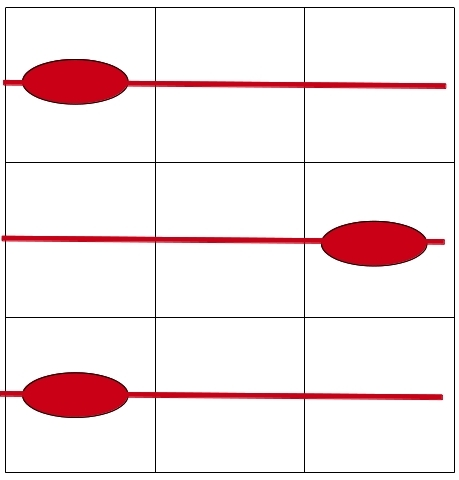
\epsfig{file=instanciaposible_ej3_out3.jpg, scale=0.15} % segunda imagen colocada a la derecha
\caption{Salida de la instancia posible Nº3.}
\label{fig-tc2}
\end{center}
\end{minipage}
\hfill
\end{figure}

\item Por otra parte, resulta importante corroborar la solución en el caso en el que todos los espacios son importantes. En este caso particular no existe solución ya que no podrían pasar dos lásers por el mismo casillero especial sin que uno de estos toque a otro láser.\newline

\textbf{Parámetro de entrada:} 
$$3\ \ 3$$
$$2\ \ 2\ \ 2$$
$$2\ \ 2\ \ 2$$
$$2\ \ 2\ \ 2$$
\textbf{Parámetro de salida:} $$-1$$\newline

\begin{center}
\begin{figure}[H] % indico que voy a poner una figura y [h] indica que la posición relativa, tambien puedo usar t = top entre otros.
\begin{minipage}[t]{.45\textwidth}
\begin{center}
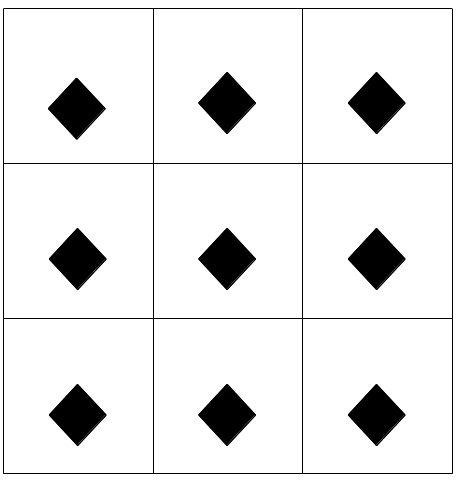
\epsfig{file=instanciaposible_ej3_in4.jpg, scale=0.13} % primera imagen colocada a la izquierda
\caption{Entrada de la instancia posible Nº4.}
\end{center}
\label{fig-tc1}
\end{minipage}
\end{figure}
\item Por otra parte, probamos el programa para un museo conformado únicamente por paredes, en otras palabras, el caso vacío. Lo relevante de este caso es que nuestro algoritmo lo considera y otorga, como salida, que la solución es no colocar ningún láser.\newline
\end{center}

\item Otra situación posible es en la que se encuentran alternados los casilleros de piso y pared. De este caso puede destacarse que no es posible aplicar ninguna de las podas mencionadas.\newline
\textbf{Parámetro de entrada:} 
$$3\ \ 3$$
$$1\ \ 0\ \ 1$$
$$0\ \ 1\ \ 0$$
$$1\ \ 0\ \ 1$$
\textbf{Parámetro de salida:} 
$$5\ \ 20000$$
$$2\ \ 0\ \ 0$$
$$2\ \ 0\ \ 2$$
$$2\ \ 1\ \ 1$$
$$2\ \ 2\ \ 0$$
$$2\ \ 2\ \ 2$$

\begin{figure}[H] % indico que voy a poner una figura y [h] indica que la posición relativa, tambien puedo usar t = top entre otros.
\hfill
\begin{minipage}[t]{.45\textwidth}
\begin{center}

\epsfig{file=instanciaposible_ej3_in5.jpg, scale=0.15} % primera imagen colocada a la izquierda
\caption{Entrada de la instancia posible Nº5.}
\label{fig-tc1}
\end{center}
\end{minipage}
\hfill
\begin{minipage}[t]{.45\textwidth}
\begin{center}
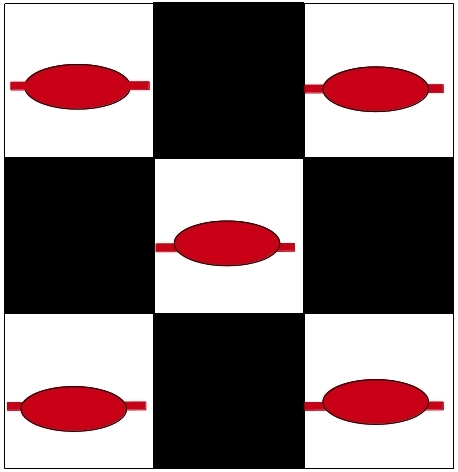
\epsfig{file=instanciaposible_ej3_out5.jpg, scale=0.15} % segunda imagen colocada a la derecha
\caption{Salida de la instancia posible Nº5.}
\label{fig-tc2}
\end{center}
\end{minipage}
\hfill
\end{figure}

\item Por último, se encuentra el caso en el que coexisten los 3 tipos de casilleros, siendo éste el mas típico del problema. \newline

\textbf{Parámetro de entrada:} 
$$3\ \ 3$$
$$1\ \ 1\ \ 1$$
$$1\ \ 2\ \ 0$$
$$0\ \ 0\ \ 1$$
\textbf{Parámetro de salida:} 
$$3\ \ 14000$$
$$1\ \ 0\ \ 1$$
$$2\ \ 1\ \ 0$$
$$2\ \ 2\ \ 2$$
\newline
\end{itemize}

\begin{figure}[H] % indico que voy a poner una figura y [h] indica que la posición relativa, tambien puedo usar t = top entre otros.
\hfill
\begin{minipage}[t]{.45\textwidth}
\begin{center}
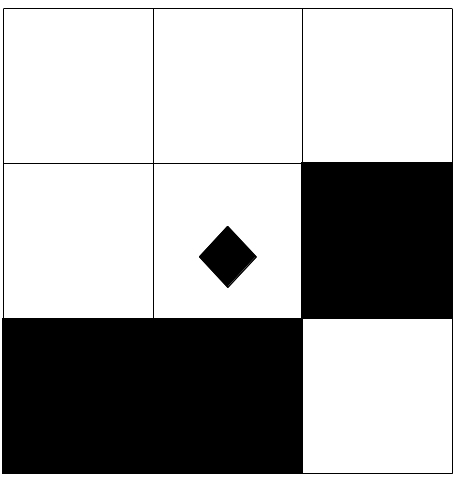
\epsfig{file=instanciaposible_ej3_in6.jpg, scale=0.15} % primera imagen colocada a la izquierda
\caption{Entrada de la instancia posible Nº6.}
\label{fig-tc1}
\end{center}
\end{minipage}
\hfill
\begin{minipage}[t]{.45\textwidth}
\begin{center}
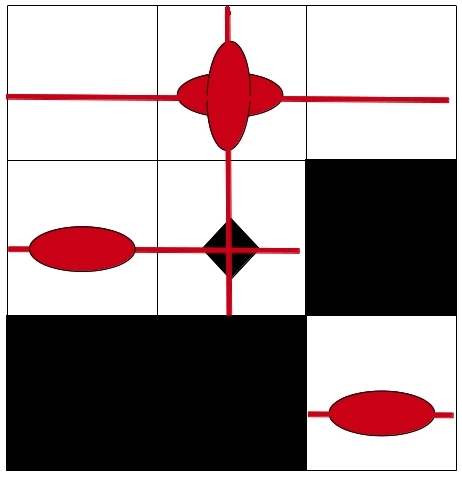
\epsfig{file=instanciaposible_ej3_out6.jpg, scale=0.15} % segunda imagen colocada a la derecha
\caption{Salida de la instancia posible Nº6.}
\label{fig-tc2}
\end{center}
\end{minipage}
\hfill
\end{figure}

\subsection{Testing}
Para realizar las pruebas de complejidad, generamos instancias aleatorias de pesos de cajas alterando la cantidad de las mismas pero manteniendo estático el peso máximo de carga de los camiones en 120 \unit{kg}. Estas instancias fueron generadas en $C++$ con la función $rand()$ de forma tal a poder acotarlas por la capacidad de carga de los camiones. La cantidad de cajas generadas se comprendió entre 5000 y 100000, agregando de a 5000 en cada iteración. De este modo, logramos medir las pruebas de nuestro algoritmo para comprobar que la complejidad correspondiera con la mencionada anteriormente.

